\documentclass[aip, cp, amsmath, amssymb, reprint, nofootinbib]{revtex4-2}

\usepackage{graphicx}
\usepackage{dcolumn}
\usepackage{bm}

\usepackage{setspace}
\usepackage{graphicx}% Include figure files
\usepackage{fancyhdr}
\setlength{\parindent}{0in}

% Page Formatting
\pagenumbering{arabic} %\pagenumbering{gobble}
\onehalfspacing %doublespacing
\pagestyle{fancy}
%\usepackage{pdfpages}

% Heading Formatting
\headheight 32pt

% Link Formatting
\usepackage{hyperref}
\hypersetup{
	colorlinks,
	allcolors=black
	%citecolor=black,
	%filecolor=black,
	%linkcolor=black,
	%urlcolor=black
}


\usepackage{csvsimple}
\usepackage{mdframed}

\definecolor{commentsColor}{rgb}{0.497495, 0.497587, 0.497464}
\definecolor{keywordsColor}{rgb}{0.541176, 0.168627, 0.886275}
\definecolor{stringColor}{rgb}{0.000000, 0.558215, 0.135316}

% Code Formatting
\usepackage{listings}
\lstset
{ %Formatting for code
	basicstyle=\footnotesize\ttfamily,
	numbers=left,
	%caption={},
	%title={},
	stepnumber=1,
	showstringspaces=false,
	tabsize=1,
	breaklines=true,
	breakatwhitespace=false,
	frame=lines,
	xleftmargin=2em,
	framexleftmargin=1.5em,
	commentstyle=\color{commentsColor}\ttfamily,
  	stringstyle=\color{stringColor}\ttfamily,
	keywordstyle=\color{keywordsColor}\bfseries,
}
\newcommand{\lstprompt}{>\!>\!>}
\newcommand{\numberwithprompt}[1]{\footnotesize\ttfamily\selectfont \lstprompt}


% https://tex.stackexchange.com/questions/340232/how-insert-a-character-at-the-begin-of-every-line-from-a-source-code
\lstdefinestyle{console} {
	basicstyle=\footnotesize\ttfamily,
	numbers=left,
	stepnumber=1,
	showstringspaces=false,
	tabsize=1,
	breaklines=true,
	breakatwhitespace=false,
	frame=single,
	xleftmargin=2em,
	framexleftmargin=2.5em,
	%backgroundcolor=\color{gray!55},
	numberstyle=\numberwithprompt,
	}

% \lstdefinelanguage{psuedocode}{
%   keywords={typeof, new, true, false, catch, function, return, null, catch, switch, var, if, in, while, do, else, case, break},
%   keywordstyle=\color{blue}\bfseries,
%   ndkeywords={class, export, boolean, throw, implements, import, this},
%   ndkeywordstyle=\color{darkgray}\bfseries,
%   identifierstyle=\color{black},
%   sensitive=false,
%   comment=[l]{//},
%   morecomment=[s]{/*}{*/},
%   commentstyle=\color{purple}\ttfamily,
%   stringstyle=\color{red}\ttfamily,
%   morestring=[b]',
%   morestring=[b]"
% }

%\usepackage{algpseudocodex}
%Book Stuff

%\usepackage{algorithm}
%\usepackage[noend]{algpseudocode}
%\makeatletter
%\def\BState{\State\hskip-\ALG@thistlm}
%\makeatother

% Figures & Drawings
\usepackage{graphicx, caption}
\usepackage{animate}
\usepackage{tikz}
\usepackage{float}
\usepackage{pict2e}
\usepackage{subcaption}

% Physics
\usepackage{physics}

% Mathematics
\usepackage{amsmath}
\usepackage{amssymb}
\usepackage{amsthm}
\usepackage{mathtools}
%\usepackage{upgreek} % More Greek letters

% I don't really know what this is but I don't want to break shit
\usepackage{aliascnt}
\newaliascnt{eqfloat}{equation}
\newfloat{eqfloat}{h}{eqflts}
\floatname{eqfloat}{Equation}
\newcommand*{\ORGeqfloat}{}
\let\ORGeqfloat\eqfloat
\def\eqfloat{%
	\let\ORIGINALcaption\caption
	\def\caption{%
		\addtocounter{equation}{-1}%
		\ORIGINALcaption
	}%
	\ORGeqfloat
}
%}

% Bibliography (Citations) Formatting

%\usepackage{cite}
\usepackage{caption}
%\usepackage[backend=bibtex,style=verbose-trad2]{biblatex}
%works really really well, but no MLA format
%\usepackage[backend=biber]{biblatex}
%\bibliographystyle{apsrev4-1}
%\usepackage[backend=biber,style=mla]{biblatex} %Doesn't print all sources for some reason


%\usepackage{graphicx}% Include figure files
\usepackage{dcolumn}% Align table columns on decimal point
\usepackage{bm}% bold math
%\usepackage[mathlines]{lineno}% Enable numbering of text and display math
%\linenumbers\relax % Commence numbering lines

\usepackage[utf8]{inputenc}
\usepackage[T1]{fontenc}
%% Loads a Times-like font. You can also load
%% {newtxtext,newtxtmath}, but not {times}, 
%% {txfonts} nor {mathtpm} as these packages
%% are obsolete and have been known to cause problems.
\usepackage{mathptmx} 


\usepackage{amsthm}
% Tikz Packages
\usepackage{circuitikz}


\tikzset{>=latex} % for LaTeX arrow head
\colorlet{myred}{red!85!black}
\colorlet{mydarkred}{red!55!black}
\colorlet{mylightred}{red!85!black!12}
\colorlet{myfieldred}{mydarkred!5} % for S' background
\colorlet{myredhighlight}{myred!20} % highlights simultaneity in ladder paradox
\colorlet{myblue}{blue!80!black}
\colorlet{mydarkblue}{blue!50!black}
\colorlet{mylightblue}{blue!50!black!30}
\colorlet{mylightblue2}{myblue!10}
\colorlet{mygreen}{green!80!black}
\colorlet{mypurple}{blue!40!red!80!black}
\colorlet{mydarkgreen}{green!50!black}
\colorlet{mydarkpurple}{blue!40!red!50!black}
\colorlet{myorange}{orange!40!yellow!95!black}
\colorlet{mydarkorange}{orange!40!yellow!85!black}
\colorlet{mybrown}{brown!20!orange!90!black}
\colorlet{mydarkbrown}{brown!20!orange!55!black}
\colorlet{mypurplehighlight}{mydarkpurple!20} % highlights simultaneity in ladder paradox
\tikzstyle{world line}=[myblue!40,line width=0.3]
\tikzstyle{world line t}=[mypurple!50!myblue!40,line width=0.3]
\tikzstyle{world line'}=[mydarkred!40,line width=0.3]
\tikzstyle{mysmallarr}=[-{Latex[length=3,width=2]},thin]
\tikzstyle{mydashed}=[dash pattern=on 3 off 3]
\tikzstyle{rod}=[mydarkbrown,draw=mydarkbrown,double=mybrown,double distance=2pt,
                 line width=0.2,line cap=round,shorten >=1pt,shorten <=1pt]
%\tikzstyle{rod'}=[rod,draw=mydarkbrown!80!red!85,double=mybrown!80!red!85]
\tikzstyle{vector}=[->,line width=1,line cap=round]
\tikzstyle{vector'}=[vector,shorten >=1.2]
\tikzstyle{particle}=[mygreen,line width=0.9]
\tikzstyle{photon}=[-{Latex[length=5,width=4]},myorange,line width=0.8,decorate,
                    decoration={snake,amplitude=1.0,segment length=5,post length=5}]

\def\tick#1#2{\draw[thick] (#1) ++ (#2:0.06) --++ (#2-180:0.12)}
\def\tickp#1#2{\draw[thick,mydarkred] (#1) ++ (#2:0.06) --++ (#2-180:0.12)}
\def\Nsamples{100} % number samples in plot
% Custom Symbols 
%{
\newcommand\halmos{\rule{.36em}{2ex}} % Custom QED Symbol
\def\contradict{\tikz[baseline, x=0.22em, y=0.22em, line width=0.032em]\draw (0,2.83)--(2.83,0) (0.71,3.54)--(3.54,0.71) (0,0.71)--(2.83,3.54) (0.71,0)--(3.54,2.83);}
\renewcommand{\qedsymbol}{\halmos}
\renewenvironment{proof}{{\bfseries \textit{Proof} \\}}{\qedsymbol}

\makeatletter
\newcommand{\crossout}[1]{% Crosses out symbol
	\begingroup
	\settowidth{\dimen@}{#1}%
	\setlength{\unitlength}{0.05\dimen@}%
	\settoheight{\dimen@}{#1}%
	\count@=\dimen@
	\divide\count@ by \unitlength
	\begin{picture}(0,0)
		\put(0,0){\line(20,\count@){20}}
		\put(0,\count@){\line(20,-\count@){20}}
	\end{picture}%
	#1%
	\endgroup
}
%}

% Mathematics (General)
\newtheorem{theorem}{Theorem}[section]
\newtheorem{corollary}{Corollary}[theorem]
\newtheorem{lemma}[theorem]{Lemma}

\newcommand{\lemref}[1]{\textit{Lemma \ref{#1}}}
\newcommand{\thmref}[1]{\textbf{Theorem \ref{#1}}}
\newcommand{\colref}[1]{\textit{Corollary \ref{#1}}}

% Physics (Quantum Mechanics)
\newcommand{\expectation}[1]{\langle{#1}\rangle}

% Physics (Electrodynamics)
\newcommand{\del}{\overline{\nabla}}
\usetikzlibrary{arrows}
%Script r (scalar)
\newcommand{\rc}{%
\resizebox{!}{1.25ex}{%
    \begin{tikzpicture}[>=round cap]
        \clip (0.09em,-0.05ex) rectangle (0.61em,0.81ex);
        \draw [line width=.11ex, <->, rounded corners=0.13ex] (0.1em,0.1ex) .. controls (0.24em,0.4ex) .. (0.35em,0.8ex) .. controls (0.29em,0.725ex) .. (0.25em,0.6ex) .. controls (0.7em,0.8ex) and (0.08em,-0.4ex) .. (0.55em,0.25ex);
    \end{tikzpicture}%
}%
}

%Script r (vector)
\newcommand{\brc}{%
\resizebox{!}{1.3ex}{%
    \begin{tikzpicture}[>=round cap]
        \clip (0.085em,-0.1ex) rectangle (0.61em,0.875ex);
        \draw [line width=.2ex, <->, rounded corners=0.13ex] (0.1em,0.1ex) .. controls (0.24em,0.4ex) .. (0.35em,0.8ex) .. controls (0.29em,0.725ex) .. (0.25em,0.6ex) .. controls (0.7em,0.8ex) and (0.08em,-0.4ex) .. (0.55em,0.25ex);
    \end{tikzpicture}%
}%
}

%Script r with a hat (unit vector)
\newcommand{\hrc}{\hat{\brc}}


% Document (General)
\newcommand{\figref}[1]{Fig. \ref{#1}}
\newcommand{\source}[1]{\caption*{Source: {#1}} }



% ========================================= %
% LaTeX Template by Aditya K. Rao
% Contact at adi.rao@mail.utoronto.ca

% Change for each document [!!!]
\newcommand\course{PHY426}	% Course Code [!!!]txt
\newcommand\doctitle{Proposed Improvements \& Additions to Schlieren Experiment} % Report Title [!!!]
\newcommand\firstauthorname{Aditya K. Rao}
\newcommand\firstauthorstdnum{Student Number: 1008307761}
\newcommand\firstauthoremail{adi.rao@mail.utoronto.ca}
%\newcommand\secondauthorname{Author Two}
%\newcommand\secondauthorstdnum{Student Number: 0000000000}
%\newcommand\secondauthoremail{report.author@mail.utoronto.ca}
\newcommand\advname{B. Braverman\space} % Advisor Name [!!!]  
\newcommand\taname{A. Sloan\space} % Advisor Name [!!!] 
\newcommand\lponename{Jack Wang\space}
\newcommand\lptwoname{Yiheng Wang\space}
\newcommand\lpthreename{Kai Lyu\space}  
\newcommand{\location}{MP222} % Location [!!!]
% ========================================= %
 
% ============== EQUIPMENT ================ %

\newcommand{\oscope}{\texttt{DSOX1202G}\space}
\newcommand{\pdiode}{\texttt{DET36A2}\space}
\newcommand{\hene}{\texttt{HNLS008L}\space}
\newcommand{\cam}{\texttt{Alium 1800 U-500}\space}

% ========================================= %


\renewcommand{\abstractname}{Overview.}
%\pagenumbering{gobble}
\usepackage{listings}

\renewcommand\lstlistingname{Code Reference}
\renewcommand\lstlistlistingname{Code Reference}
\usepackage{tikz}
\usetikzlibrary{patterns}

\usepackage{circuitikz}

%\addbibresource{references.bib}
\usepackage{lipsum}
\usetikzlibrary{calc}

\begin{document}
\onecolumngrid
\pagenumbering{arabic}
\title{\doctitle}
\author{\firstauthorname}
\email{\firstauthoremail}
\thanks{\firstauthorstdnum}

%\author{\lponename}
%\author{\lptwoname}
%\author{\lpthreename}

%\email{report.author@mail.utoronto.ca}
%\thanks{Student Number: 0000000000}
\affiliation{
University of Toronto \\
\location, 60 St. George Street, Toronto, Ontario M5S 1A7, Canada.% Force line breaks with \\ if necessary
}

\date{\today} %Put in date of submission [!!!]

\preprint{APS/123-QED}
\begin{abstract}
    For this improvement report, the author has opted to focus on improvements related to the Schlieren Imaging laboratory. In paritcular, these improvements revolve around the addition of a new experiment to image free convection in air. All of the apparatus required for this experiment is available in APL. The author has also provided a new method of data processing for the convection current experiment. This method, while not fully developed, shows promise and may be of use to future students. There are some furhter general improvements to the setup also included.
\end{abstract}

    \maketitle
    %\tableofcontents 

    \lhead{\firstauthorname\vspace{0.1cm}}
    \chead{\textbf{\course} \\ \doctitle}
    \rhead{\textbf{Prof:} \advname \\ \textbf{TA:} \taname}
    \nocite{*}
    %\newpage
    %\twocolumngrid
    % \section{Experimental Setup}
    %     Improvements to the experimental setup range from the inclusion of additional apparatus to simply the removal of (semi) redudant equipment. A simple modification is directly imaging into the camera instead of using a reflecting mirror. Not only does this reduce the `smearing' effect caused by reflecting through the mirror, but more light also enters the camera sensor reducing the required exposure time.  
    % \subsection{New Apparatus}
    %     \subsubsection{Color Filters}
    %         The inclusion of color filters would allow for dual color Schlieren imaging. This would allow for the visualization of different temperature gradients in the same image. This would be useful for the convection current experiment.
    %     \subsubsection{Improved Water Heater}
    %         Currently an aquarium water heater with minimal temperature control is provided to generate convection currents in the tank. The accuracy of this device is questionable, a more accurate water heater would be benificial for more fine tuning of the temperature gradients generated in the tank.
    %     \subsubsection{Different Color Light Source}
    %         The inclusion of a laser Schlieren deflectometry setup would allow for the visualization of the refractive index gradient in a medium. This would be useful for the convection current experiment as well as other experiments.
    %     \subsubsection{Laser Schlieren Deflectometry}
    %         The inclusion of a laser Schlieren deflectometry setup would allow for the visualization of the refractive index gradient in a medium. This would be useful for the convection current experiment as well as other experiments.
    %     \subsection{Modification to Existing Setup}
    %         \subsubsection{Rail Mount for Mirrors}
    %             Adding a rail mount to \texttt{\#M2} would not only allow more precise control over the measurement system, but also allow the student to investigate the effect of different reflection angles on the Schlieren image. Prof. H. Kleine (UNSW)\footnote{The author and Prof. Kleine interacted over email regarding this issue.}\cite{kleine} stated that the accepted upperbound for such a setup is approximately 7\% while the current setup seems to be more than this upper bound. The result was a significant astigmatism leading to a reduced effective of the knife edge. 
    %             The rail mount would also allow students to investigate the results of such astigmatism.
    %         \subsubsection{Higher Quality Tank}
    %             Currently, the water tank used for the convection current experiment seems to be standard aquarium tank glass. The problem with such a setup is the resultant reduction in quality, as suggested by both Prof. H. Kleine (UNSW) \cite{kleine} and Settles \cite{settles_2013}
    % \section{Laboratory Manual}
    %     The time table in the laboratory manual is quite useful, however, is somewhat unrealistic. It take, at times, significantly longer to setup up the convection current experiment. Instead, a selection of expriment should be provided similar to that in the \texttt{LENS} lab manual. Additionally, the diagrams in the manual would benifit from further explinations. Specifically, significant improvements may be made to the `theory' section of the manual. Some images the author has created are provided in the appendix should they be of use for improvements to the manual.
    \vspace{-2cm}
    \section{Modification to Existing Setup}
        \subsection{Imaging Directly into Camera}
        Currently the experimental setup suggested in the laboratory manual is good but could be significantly improved with some minor modification to existing equipment as well as the addition of a few minor components. 

        The first trivial modification is to directly image into the camera instead of using a reflecting mirror. Not only does this reduce the `smearing' effect caused by reflecting through the mirror, but more light also enters the camera sensor reducing the required exposure time. This is illustrated in \figref{fig:direct-image}. 

        \begin{figure}[H]
            \centering
            \begin{subfigure}{0.49\linewidth}
                \centering
                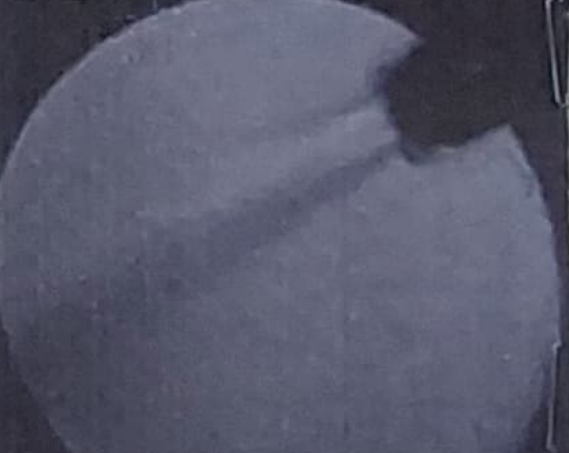
\includegraphics[width=0.5\linewidth]{figures/pre.png}
                %\input{figures/pre.png}
                \caption{Sample image without proposed modifications.}
                \label{fig:direct-image}
            \end{subfigure}
            \begin{subfigure}{0.49\linewidth}
                \centering
                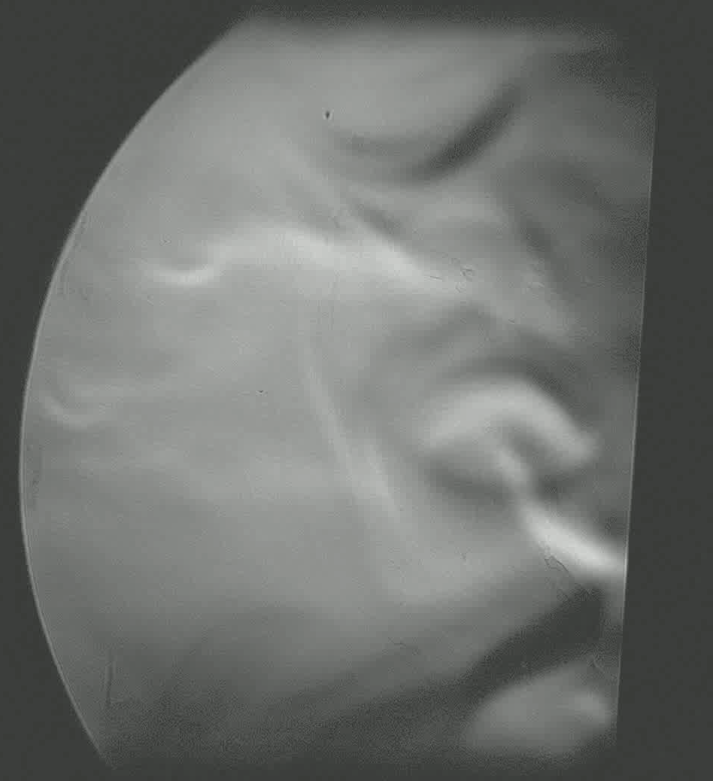
\includegraphics[width=0.4\linewidth, angle=-90]{figures/sampleC.png}
                \caption{Sample image with proposed modification}
                \label{fig:freeconvection}
            \end{subfigure}
            \caption{Images before (a) and after (b) the modifications. Image (a) is of the heat gun proposed in the lab manual \cite{manual} while image (b) is of the proposed free convection experiment.}
        \end{figure}

        Though there is the concern of damaging the camera sensor at high enough LED settings, this can be mitigated through proper instruction to students (sufficient warnings in laboratory manual). A few more major benifits include that less light is needed from the LED, eliminating the requirement that the room be entirely dark. Additionally, the need for tinkering with the basedcam2 settings is effectively eliminated allowing students to focus on the phenomena they're imaging.

        \subsection{Addition of Rail Mounts for Mirrors}
        Adding a rail mount to \texttt{\#M2} would not only allow more precise control over the measurement system, but also allow the student to investigate the effect of different reflection angles on the Schlieren image. Prof. H. Kleine (UNSW)\footnote{The author and Prof. Kleine interacted over email regarding this issue.}\cite{kleine} stated that the accepted upperbound for such a setup is approximately $7^{\circ}$ while the current setup seems to be more than this upper bound. The result was a significant astigmatism leading to a reduced effective of the knife edge. 

        \begin{figure}[H]
            \centering
            \scalebox{0.9}{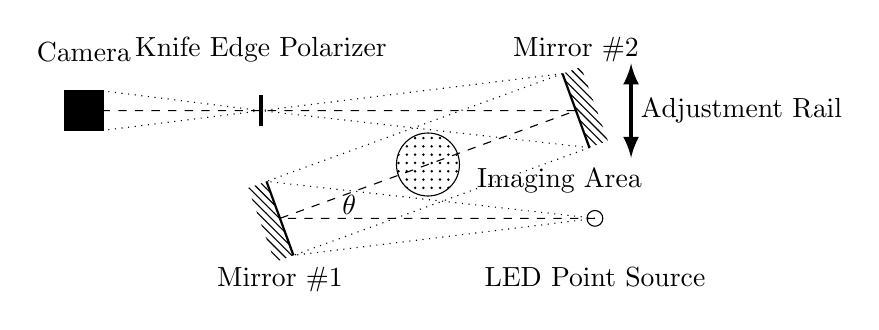
\begin{tikzpicture}
    \def\angle{-70}
    \def\dist{4}

    \begin{scope}[rotate=\angle]
        \coordinate(mA1) at (-0.5,-\dist/2);
        \coordinate(mA2) at (0.5,-\dist/2);
        \coordinate(mA) at (0,-\dist/2);

        \coordinate(mB1) at (-0.5,\dist/2);
        \coordinate(mB2) at (0.5,\dist/2);
        \coordinate(mB) at (0,\dist/2);

        \draw[thick] (mA1) -- (mA2);
        \fill[pattern=north west lines, draw=none] (mA1) rectangle ($(mA2)+(0,-0.25)$);

        \draw[thick] (mB1) -- (mB2);
        \fill[pattern=north west lines, draw=none] (mB1) rectangle ($(mB2)+(0,0.25)$);

        \draw[dotted] (-0.5,\dist/2) -- (-0.5,-\dist/2);
        \draw[dotted] (0.5,\dist/2) -- (0.5,-\dist/2);
    \end{scope}


    \coordinate (led) at ($(mA)+(\dist,0)$);
    \coordinate (ke) at ($(mB)-(\dist,0)$);
    \coordinate (cam) at ($(ke)-(\dist/2,0)$);
    \coordinate (cam1) at ($(cam)+(0,0.25)$);
    \coordinate (cam2) at ($(cam)+(0,-0.25)$);

    \draw[dotted] (led) -- (mA1);
    \draw[dotted] (led) -- (mA2);

    \draw[dotted] (mB1) -- (ke);
    \draw[dotted] (mB2) -- (ke);

    \draw[dashed] (led) -- (mA) -- (mB) -- (ke) -- (cam);

    \draw[ultra thick] ($(ke)+(0,0.2)$) -- ($(ke)+(0,-0.2)$);

    \draw (led) circle (0.1);
    
    \draw[fill=black] ($(cam1)+(-0.5,0)$) rectangle ($(cam2)$);


    \draw[dotted] (ke) -- (cam1);
    \draw[dotted] (ke) -- (cam2);

    \draw[color=black, pattern=dots] (0,0) circle (0.4)node[anchor=west, shift={(0.5,-0.2)}]{Imaging Area};

    \draw[ultra thick, ->] ($(mB) + (0.7,0)$) -- ($(mB) + (0.7,0.6)$);
    \draw[ultra thick, ->] ($(mB) + (0.7,0)$) -- ($(mB) - (-0.7,0.6)$);
    \draw ($(mB) + (0.7,0)$)node[anchor=west]{Adjustment Rail};
    \draw (mA)node[xshift=25, yshift=5]{$\theta$};

    % Labels
    \node[anchor=north, shift={(0,-0.5)}] at (mA) {Mirror \#1};
    \node[anchor=south, shift={(0,0.5)}] at (mB) {Mirror \#2};
    \node[anchor=north, shift={(0,-0.5)}] at (led) {LED Point Source};
    \node[anchor=south, shift={(0,0.5)}] at (ke) {Knife Edge Polarizer};
    \node[anchor=south, shift={(0,0.5)}] at ($(cam)+(-0.25,0)$) {Camera};
\end{tikzpicture}}
            \caption{Improved diagram of the experimental setup. Modification to setup also included in the diagram. Adjustment rail would effectively change the angle of the mirror $\theta$ allowing for more precise control over the system.}
        \end{figure}

        The rail mount would also allow students to investigate the results of such astigmatism should they be more interested in improving the experimental setup rather than conducting a specific experiment. This also allows for further connections with the `lens' experiment should the student be interested in investigating the differences with the single mirror schlieren setup in the \texttt{LENS} lab.

    \section{Investigation of Free Convection In Air}
        Currently the laboratory manual focuses only one imaging convection currents with minor forays to other related areas. The method of Schleiren Imaging is incredibly versatile and interesting, even to students not explicetly interested in fluid dynamics. One experiment that was conducted by the author to investigate free convection in air \cite{adi} is outlined in the following section. The new data analysis procedure used by the author is outlined in the later section on Data Processing. This experiment was proposed to the author by Prof. B. Braverman duing the \texttt{PHY424} lab \cite{pbrave}.

        In this proposed extension, the author investigated free convection in air using a metal fin heated to high temperatures. The experimental setup is shown in \figref{fig:freeconvectionfin}. The experiment was conducted using a hotplate to heat the metal fin and a thermocouple \cite{fluke} to record the temperature difference. The metal fin was placed in the imaging area and heated to high temperatures using a hotplate. To isolate heat to just the fins surface, insulating foam was placed beside the fin.

        The objective of this experiment was to observe the transition between laminar and turbulent flow at the boundary layer of a heated metal fin. With the prediction that, at low temperatures, the flow would produce a laminar flow pattern and at high temperatures, the flow would produce a turbulent flow pattern. These patterns being generated through taking a slice of each frame of the evolution and comparing it to the rest of the evolution.


        \begin{figure}[H]
            \centering
            \scalebox{0.7}{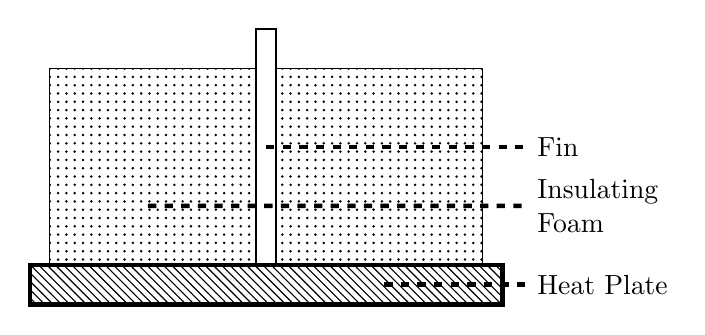
\begin{tikzpicture}
    \def\width{6}
    \def\height{3}
    \def\fmheight{2.5}
    \def\thick{0.25}
    \def\hpthick{0.5}

    \coordinate (LC) at ($(0,0) + (-\width/2, \hpthick/2)$);
    \coordinate (RC) at ($(0,0) + (\width/2, \hpthick/2)$);

    \coordinate (FINBASE) at ($(0,0) + (0,\hpthick/2)$);

    % Hot Plate
    \draw[ultra thick, pattern=north west lines] (LC) rectangle ($(RC)-(0,\hpthick)$);

    % Fin Body
    \draw[thick] ($(FINBASE)-(\thick/2,0)$) rectangle ($(FINBASE)+(\thick/2,\height)$);

    % Foam Left
    \draw[pattern=dots] ($(LC)+(0.25,0)$) rectangle ($(FINBASE)+(-\thick/2,\fmheight)$);

    % Foam Right
    \draw[pattern=dots] ($(FINBASE)+(\thick/2,\fmheight)$) rectangle ($(RC)-(0.25,0)$);

    % Labels
    \draw[ultra thick, dashed] ($(FINBASE)+(0,\height/2)$) -- ($(FINBASE)+(\width/2+0.3,\height/2)$)node [anchor=west] {Fin};

    \draw[ultra thick, dashed] ($(LC)+(\width/4,\fmheight/2 -0.5)$) -- ($(\width/2+0.3,\fmheight/2 + \hpthick/2 -0.5)$)node [anchor=west, text width=1.5cm] {Insulating Foam};

    \draw[ultra thick, dashed] ($(RC)-(\width/4,\hpthick/2)$) -- ($(\width/2+0.3,0)$)node [anchor=west] {Heat Plate};
\end{tikzpicture}}
            \caption{Experimental setup for measuring free convection in air. The metal fin was placed in the imaging area and heated to high temperatures using a hotplate. To isolate heat to just the fins surface, insulating foam was placed beside the fin.}
            \label{fig:freeconvectionfin}
        \end{figure}

        The output image of the experiment is shown in \figref{fig:freeconvection}. There are a variety of ways that students may analyse this data. The author proposes the `pixel-slice' method outlined in the following section.


    \section{Data Processing}
        A different method of data processing could be used to investigate free convection as a `timeseries' data. For every frame, one, or multiple, `pixel slice' were taken at the same set of points. This is better illustrated in \figref{fig:slice-1}. These slices could then be aggregated to for a `timeseries' of the data, in effect, showing the changes in temperature at each point over time, this is better illustrated in \figref{fig:slice-2}.

        \begin{figure}[H]
            \centering
            \begin{subfigure}{0.49\linewidth}
                \centering
                \scalebox{1.2}{
                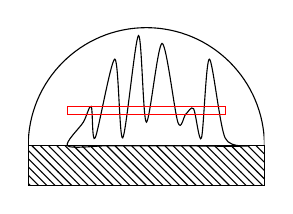
\begin{tikzpicture}

    \begin{scope}
        \clip (-1.5,0) rectangle (1.5,1.5);
        \draw (0,0) circle(1.5);
        \draw (-1.5,0) -- (1.5,0);
    \end{scope}

    \draw [black] plot [smooth cycle] coordinates {(0,0) (-0.5,0) (-1,0) (-0.8,0.3) (-0.7,0.5) (-0.65,0.1) (-0.4,1.1) (-0.3,0.1) (-0.1,1.4) (0,0.3) (0.2,1.3) (0.4,0.3) (0.5,0.4) (0.6,0.47) (0.7,0.1) (0.8,1.1) (1,0.1) (1.3,0) (0.5,0) (1,0) (0,0)};

    \draw[red] (-1, 0.5) rectangle (1, 0.4);

    \draw[pattern=north west lines] (-1.5,0) rectangle (1.5,-0.5);

\end{tikzpicture}}
                \caption{Sketch of pixel slice on free convection fin data, red area is where the box is sampled from.}
                \label{fig:slice-1}
            \end{subfigure}
            \begin{subfigure}{0.49\linewidth}
                \centering
                \scalebox{1.2}{
                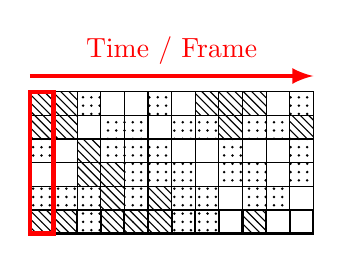
\begin{tikzpicture}
    \def\boxwidth{0.3}

    \coordinate (Row1) at (0,0);
    \coordinate (Row2) at (0,\boxwidth);
    \coordinate (Row3) at (0,2*\boxwidth);
    \coordinate (Row4) at (0,3*\boxwidth);
    \coordinate (Row5) at (0,4*\boxwidth);
    %\coordinate (Row5) at (0,5*\boxwidth);

    % Layer 1
    \draw[thick, pattern=north west lines] (0,0) rectangle (\boxwidth, \boxwidth);
    \draw[pattern=dots] (0,\boxwidth) rectangle (\boxwidth, 2*\boxwidth);
    \draw[fill=white] (0,2*\boxwidth) rectangle (\boxwidth, 3*\boxwidth);
    \draw[pattern=dots] (0,3*\boxwidth) rectangle (\boxwidth, 4*\boxwidth);
    \draw[pattern=north west lines] (0,4*\boxwidth) rectangle (\boxwidth, 5*\boxwidth);
    \draw[pattern=north west lines] (0,5*\boxwidth) rectangle (\boxwidth, 6*\boxwidth);


    % Layer 2
    \draw[thick, pattern=north west lines] (\boxwidth,0) rectangle (2*\boxwidth, \boxwidth);
    \draw[pattern=dots] (\boxwidth,\boxwidth) rectangle (2*\boxwidth, 2*\boxwidth);
    \draw[fill=white] (\boxwidth,2*\boxwidth) rectangle (2*\boxwidth, 3*\boxwidth);
    \draw[fill=white] (\boxwidth,3*\boxwidth) rectangle (2*\boxwidth, 4*\boxwidth);
    \draw[pattern=north west lines] (\boxwidth,4*\boxwidth) rectangle (2*\boxwidth, 5*\boxwidth);
    \draw[pattern=north west lines] (\boxwidth,5*\boxwidth) rectangle (2*\boxwidth, 6*\boxwidth);



    % Layer 3
    \draw[thick, pattern=dots] (2*\boxwidth,0) rectangle (3*\boxwidth, \boxwidth);
    \draw[pattern=dots] (2*\boxwidth,\boxwidth) rectangle (3*\boxwidth, 2*\boxwidth);
    \draw[pattern=north west lines] (2*\boxwidth,2*\boxwidth) rectangle (3*\boxwidth, 3*\boxwidth);
    \draw[pattern=north west lines] (2*\boxwidth,3*\boxwidth) rectangle (3*\boxwidth, 4*\boxwidth);
    \draw[fill=white] (2*\boxwidth,4*\boxwidth) rectangle (3*\boxwidth, 5*\boxwidth);
    \draw[pattern=dots] (2*\boxwidth,5*\boxwidth) rectangle (3*\boxwidth, 6*\boxwidth);

    

    
    % Layer 4
    \draw[thick, pattern=north west lines] (3*\boxwidth,0) rectangle (4*\boxwidth, \boxwidth);
    \draw[pattern=north west lines] (3*\boxwidth,\boxwidth) rectangle (4*\boxwidth, 2*\boxwidth);
    \draw[pattern=north west lines] (3*\boxwidth,2*\boxwidth) rectangle (4*\boxwidth, 3*\boxwidth);
    \draw[pattern=dots] (3*\boxwidth,3*\boxwidth) rectangle (4*\boxwidth, 4*\boxwidth);
    \draw[pattern=dots] (3*\boxwidth,4*\boxwidth) rectangle (4*\boxwidth, 5*\boxwidth);
    \draw[fill=white] (3*\boxwidth,5*\boxwidth) rectangle (4*\boxwidth, 6*\boxwidth);



    % Layer 5
    \draw[thick, pattern=north west lines] (4*\boxwidth,0) rectangle (5*\boxwidth, \boxwidth);
    \draw[pattern=dots] (4*\boxwidth,\boxwidth) rectangle (5*\boxwidth, 2*\boxwidth);
    \draw[pattern=dots] (4*\boxwidth,2*\boxwidth) rectangle (5*\boxwidth, 3*\boxwidth);
    \draw[pattern=dots] (4*\boxwidth,3*\boxwidth) rectangle (5*\boxwidth, 4*\boxwidth);
    \draw[pattern=dots] (4*\boxwidth,4*\boxwidth) rectangle (5*\boxwidth, 5*\boxwidth);
    \draw[fill=white] (4*\boxwidth,5*\boxwidth) rectangle (5*\boxwidth, 6*\boxwidth);


    % Layer 6
    \draw[thick, pattern=north west lines] (5*\boxwidth,0) rectangle (6*\boxwidth, \boxwidth);
    \draw[pattern=north west lines] (5*\boxwidth,\boxwidth) rectangle (6*\boxwidth, 2*\boxwidth);
    \draw[pattern=dots] (5*\boxwidth,2*\boxwidth) rectangle (6*\boxwidth, 3*\boxwidth);
    \draw[pattern=dots] (5*\boxwidth,3*\boxwidth) rectangle (6*\boxwidth, 4*\boxwidth);
    \draw[fill=white] (5*\boxwidth,4*\boxwidth) rectangle (6*\boxwidth, 5*\boxwidth);
    \draw[pattern=dots] (5*\boxwidth,5*\boxwidth) rectangle (6*\boxwidth, 6*\boxwidth);


    % Layer 7
    \draw[thick, pattern=dots] (6*\boxwidth,0) rectangle (7*\boxwidth, \boxwidth);
    \draw[pattern=dots] (6*\boxwidth,\boxwidth) rectangle (7*\boxwidth, 2*\boxwidth);
    \draw[pattern=dots] (6*\boxwidth,2*\boxwidth) rectangle (7*\boxwidth, 3*\boxwidth);
    \draw[fill=white] (6*\boxwidth,3*\boxwidth) rectangle (7*\boxwidth, 4*\boxwidth);
    \draw[pattern=dots] (6*\boxwidth,4*\boxwidth) rectangle (7*\boxwidth, 5*\boxwidth);
    \draw[fill=white] (6*\boxwidth,5*\boxwidth) rectangle (7*\boxwidth, 6*\boxwidth);



    % Layer 8
    \draw[thick, pattern=dots] (7*\boxwidth,0) rectangle (8*\boxwidth, \boxwidth);
    \draw[pattern=dots] (7*\boxwidth,\boxwidth) rectangle (8*\boxwidth, 2*\boxwidth);
    \draw[fill=white] (7*\boxwidth,2*\boxwidth) rectangle (8*\boxwidth, 3*\boxwidth);
    \draw[fill=white] (7*\boxwidth,3*\boxwidth) rectangle (8*\boxwidth, 4*\boxwidth);
    \draw[pattern=dots] (7*\boxwidth,4*\boxwidth) rectangle (8*\boxwidth, 5*\boxwidth);
    \draw[pattern=north west lines] (7*\boxwidth,5*\boxwidth) rectangle (8*\boxwidth, 6*\boxwidth);



    % Layer 9
    \draw[thick, fill=white] (8*\boxwidth,0) rectangle (9*\boxwidth, \boxwidth);
    \draw[fill=white] (8*\boxwidth,\boxwidth) rectangle (9*\boxwidth, 2*\boxwidth);
    \draw[pattern=dots] (8*\boxwidth,2*\boxwidth) rectangle (9*\boxwidth, 3*\boxwidth);
    \draw[pattern=dots] (8*\boxwidth,3*\boxwidth) rectangle (9*\boxwidth, 4*\boxwidth);
    \draw[pattern=north west lines] (8*\boxwidth,4*\boxwidth) rectangle (9*\boxwidth, 5*\boxwidth);
    \draw[pattern=north west lines] (8*\boxwidth,5*\boxwidth) rectangle (9*\boxwidth, 6*\boxwidth);


    % Layer 10
    \draw[thick, pattern=north west lines] (9*\boxwidth,0) rectangle (10*\boxwidth, \boxwidth);
    \draw[pattern=dots] (9*\boxwidth,\boxwidth) rectangle (10*\boxwidth, 2*\boxwidth);
    \draw[pattern=dots] (9*\boxwidth,2*\boxwidth) rectangle (10*\boxwidth, 3*\boxwidth);
    \draw[fill=white] (9*\boxwidth,3*\boxwidth) rectangle (10*\boxwidth, 4*\boxwidth);
    \draw[pattern=dots] (9*\boxwidth,4*\boxwidth) rectangle (10*\boxwidth, 5*\boxwidth);
    \draw[pattern=north west lines] (9*\boxwidth,5*\boxwidth) rectangle (10*\boxwidth, 6*\boxwidth);


    % Layer 11
    \draw[thick, fill=white] (10*\boxwidth,0) rectangle (11*\boxwidth, \boxwidth);
    \draw[pattern=dots] (10*\boxwidth,\boxwidth) rectangle (11*\boxwidth, 2*\boxwidth);
    \draw[fill=white] (10*\boxwidth,2*\boxwidth) rectangle (11*\boxwidth, 3*\boxwidth);
    \draw[fill=white] (10*\boxwidth,3*\boxwidth) rectangle (11*\boxwidth, 4*\boxwidth);
    \draw[pattern=dots] (10*\boxwidth,4*\boxwidth) rectangle (11*\boxwidth, 5*\boxwidth);
    \draw[fill=white] (10*\boxwidth,5*\boxwidth) rectangle (11*\boxwidth, 6*\boxwidth);


    % Layer 12
    \draw[thick, fill=white] (11*\boxwidth,0) rectangle (12*\boxwidth, \boxwidth);
    \draw[fill=white] (11*\boxwidth,\boxwidth) rectangle (12*\boxwidth, 2*\boxwidth);
    \draw[pattern=dots] (11*\boxwidth,2*\boxwidth) rectangle (12*\boxwidth, 3*\boxwidth);
    \draw[pattern=dots] (11*\boxwidth,3*\boxwidth) rectangle (12*\boxwidth, 4*\boxwidth);
    \draw[pattern=north west lines] (11*\boxwidth,4*\boxwidth) rectangle (12*\boxwidth, 5*\boxwidth);
    \draw[pattern=dots] (11*\boxwidth,5*\boxwidth) rectangle (12*\boxwidth, 6*\boxwidth);


    %\draw[color=red, ultra thick] (0,0) rectangle (12*\boxwidth, 6*\boxwidth);

    \draw[color=red, ultra thick] (0,0) rectangle (\boxwidth, 6*\boxwidth);

    \draw[color=red, ->, ultra thick] (0, 6*\boxwidth+0.2) -- (12*\boxwidth, 6*\boxwidth+0.2) node [anchor=south, midway] {Time / Frame};

\end{tikzpicture}}
                \caption{Evolution of pixel slice over time.}
                \label{fig:slice-2}
            \end{subfigure}
            \caption{Pixel slice methodology illustrations. \figref{fig:slice-1} shows the sampling of the slice while \figref{fig:slice-2} shows the evolution of the slice over time.}
        \end{figure}

        This slice methodology applied to the free convection in air experiment (outlined in the previous section) is shown in \figref{fig:slice-real} from the authors final \texttt{PHY424} report \cite{adi}.

        % \begin{figure}[H]
        %     \centering
        %     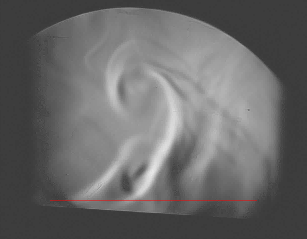
\includegraphics[width=0.8\linewidth]{figures/Pixel Slice Real.png}
        %     \caption{Pixel Slice methodology}
        %     \label{fig:slice-real}
        % \end{figure}

        \begin{figure}[H]
            \centering
            \begin{subfigure}{0.33\linewidth}
                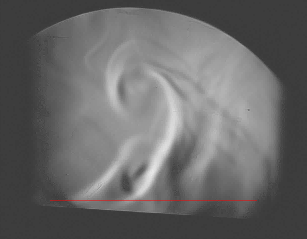
\includegraphics[width=0.5\linewidth]{figures/Pixel Slice Real.png}
                \caption{Example of pixel slice taken for free convection fin experiment.}
                \label{fig:slice-real}
            \end{subfigure}
            \begin{subfigure}[b]{0.33\linewidth}
                \centering
                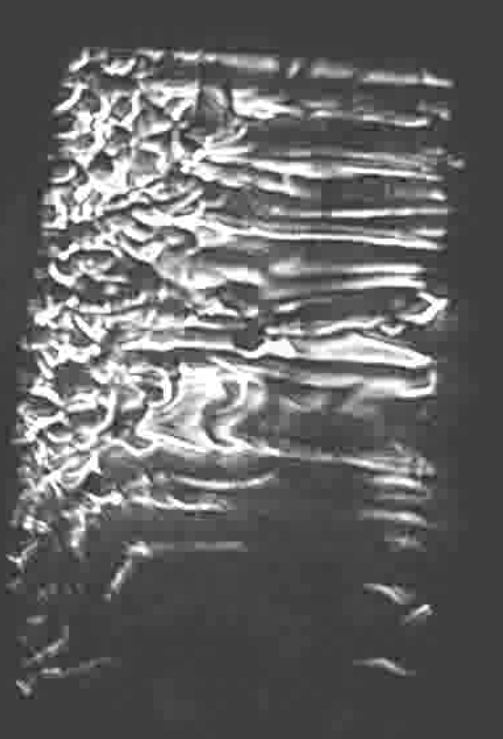
\includegraphics[width=0.47\linewidth, angle=-90]{figures/LAMINAR_RAW.png}
                \caption{Still frame of tank while being heated.}
                \label{fig:laminar1}
            \end{subfigure}
            \begin{subfigure}[b]{0.33\linewidth}
                \centering
                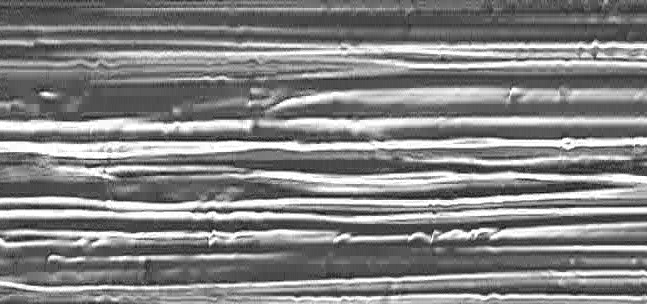
\includegraphics[width=\linewidth]{figures/DATA.LAMINAR.png}
                \caption{Evolution of pixel slice over time.}
                \label{fig:laminar2}
            \end{subfigure}
            %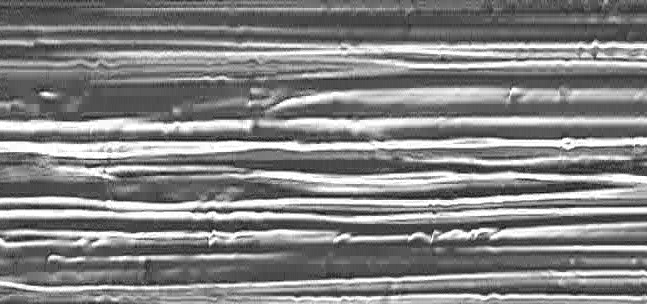
\includegraphics[width=0.9\linewidth]{figures/DATA.LAMINAR.png}
            \caption{Example of pixel slice methodology in action. \figref{fig:slice-real} shows a slice taken for the free convection experiment while \figref{fig:laminar1} and \figref{fig:laminar2} show the method applied to laminar flow data taken when trying to image convection currents.}
            \label{fig:laminar}
        \end{figure}

        This methodology was also applied to data from Rayleigh-B{\'e}nard convection current experiment outlined in the laboratory manual\cite{manual} as a test. The laminar flow of a still frame can be seen in Figure \ref{fig:laminar1} and an analysis utilizing the pixel slice method present in Figure \ref{fig:laminar2}. In this image, the white lines represent faster air mixed with slower air. Given that the `time series' data in \figref{fig:laminar2} shows a relatively regular pattern, it shows that the flow is likely laminar. 

        It should be noted that additional work needs to be done on this processing methodology, though what is provided seems to be a promising start and may be benificial to future students.

    % Line to seperate report content from acknowledgements and references
    \onecolumngrid
    \begin{center}
        \vspace{0.8cm}
        \noindent\rule{0.9\textwidth}{0.5pt}
    \end{center}

    % \begin{acknowledgments}
    %     The work conducted by the other lab partners was instrumental in this lab. Thank you to \lponename, \lptwoname, and \lpthreename for their help in setting up the equipment and conducting the experiments. Additionally, thank you to the Teaching Assistant \taname and Professor \advname for their guidance and support.
    % \end{acknowledgments}

\bibliography{references}

% \appendix
% \section{Images}
% \begin{figure}[H]
%     \centering
%     \scalebox{1.5}{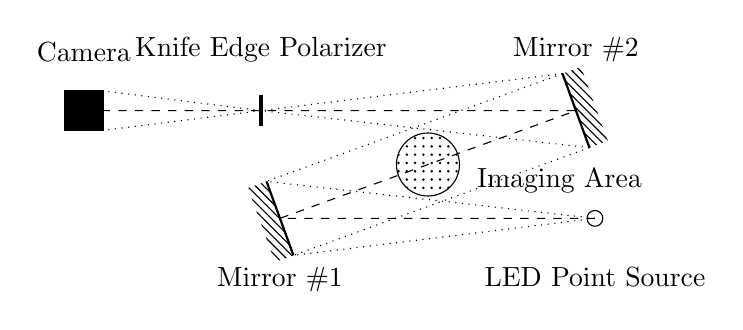
\begin{tikzpicture}
    \def\angle{-70}
    \def\dist{4}

    \begin{scope}[rotate=\angle]
        \coordinate(mA1) at (-0.5,-\dist/2);
        \coordinate(mA2) at (0.5,-\dist/2);
        \coordinate(mA) at (0,-\dist/2);

        \coordinate(mB1) at (-0.5,\dist/2);
        \coordinate(mB2) at (0.5,\dist/2);
        \coordinate(mB) at (0,\dist/2);

        \draw[thick] (mA1) -- (mA2);
        \fill[pattern=north west lines, draw=none] (mA1) rectangle ($(mA2)+(0,-0.25)$);

        \draw[thick] (mB1) -- (mB2);
        \fill[pattern=north west lines, draw=none] (mB1) rectangle ($(mB2)+(0,0.25)$);

        \draw[dotted] (-0.5,\dist/2) -- (-0.5,-\dist/2);
        \draw[dotted] (0.5,\dist/2) -- (0.5,-\dist/2);
    \end{scope}


    \coordinate (led) at ($(mA)+(\dist,0)$);
    \coordinate (ke) at ($(mB)-(\dist,0)$);
    \coordinate (cam) at ($(ke)-(\dist/2,0)$);
    \coordinate (cam1) at ($(cam)+(0,0.25)$);
    \coordinate (cam2) at ($(cam)+(0,-0.25)$);

    \draw[dotted] (led) -- (mA1);
    \draw[dotted] (led) -- (mA2);

    \draw[dotted] (mB1) -- (ke);
    \draw[dotted] (mB2) -- (ke);

    \draw[dashed] (led) -- (mA) -- (mB) -- (ke) -- (cam);

    \draw[ultra thick] ($(ke)+(0,0.2)$) -- ($(ke)+(0,-0.2)$);

    \draw (led) circle (0.1);
    
    \draw[fill=black] ($(cam1)+(-0.5,0)$) rectangle ($(cam2)$);


    \draw[dotted] (ke) -- (cam1);
    \draw[dotted] (ke) -- (cam2);

    \draw[color=black, pattern=dots] (0,0) circle (0.4)node[anchor=west, shift={(0.5,-0.2)}]{Imaging Area};

    % Labels
    \node[anchor=north, shift={(0,-0.5)}] at (mA) {Mirror \#1};
    \node[anchor=south, shift={(0,0.5)}] at (mB) {Mirror \#2};
    \node[anchor=north, shift={(0,-0.5)}] at (led) {LED Point Source};
    \node[anchor=south, shift={(0,0.5)}] at (ke) {Knife Edge Polarizer};
    \node[anchor=south, shift={(0,0.5)}] at ($(cam)+(-0.25,0)$) {Camera};
\end{tikzpicture}}
%     \caption{Improved diagram of the experimental setup.}
% \end{figure}


% \begin{figure}[H]
%     \centering
%     \scalebox{1.5}{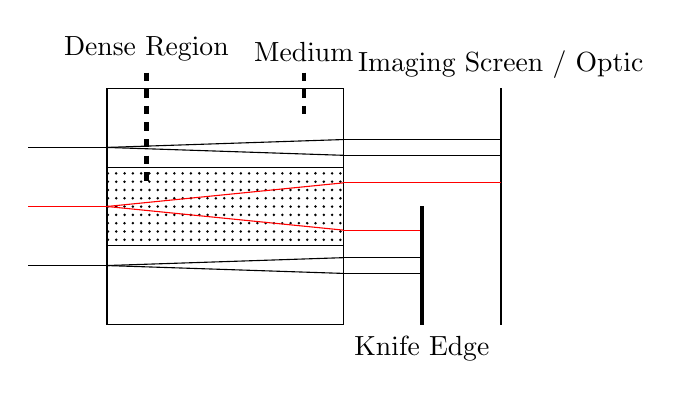
\begin{tikzpicture}
    \def\side{3}
    \def\height{3}
    \def\fmheight{2.5}
    \def\thick{0.25}
    \def\hpthick{0.5}

    \coordinate (TLC) at (-\side/2, \side/2);
    \coordinate (TRC) at (\side/2, \side/2);
    \coordinate (BLC) at (-\side/2, -\side/2);
    \coordinate (BRC) at (\side/2, -\side/2);

    \coordinate (TLC-dense) at ($(TLC)+(0,-1)$);
    \coordinate (TRC-dense) at ($(TRC)+(0,-1)$);
    \coordinate (BLC-dense) at ($(BLC)+(0,1)$);
    \coordinate (BRC-dense) at ($(BRC)+(0,1)$);

    % Draw Medium
    \draw (TLC) rectangle (BRC);

    % Dense Region
    \draw[pattern=dots] (TLC-dense) rectangle (BRC-dense);

    % Parallel Rays
    \draw ($(TLC)+(-1,-\side/4)$) -- ($(TLC)+(0,-\side/4)$);
    \draw[color=red] ($(TLC)+(-1,-\side/2)$) -- ($(TLC)+(0,-\side/2)$);
    \draw ($(TLC)+(-1,-3*\side/4)$) -- ($(TLC)+(0,-3*\side/4)$);

    % Refracting Rays
    \draw ($(TLC)+(0,-\side/4)$) -- ($(TRC)+(0,-\side/4+0.1)$);
    \draw[color=red] ($(TLC)+(0,-\side/2)$) -- ($(TRC)+(0,-\side/2+0.3)$);
    \draw ($(TLC)+(0,-3*\side/4)$) -- ($(TRC)+(0,-3*\side/4+0.1)$);

    % Refracting Rays
    \draw[color=black] ($(TLC)+(0,-\side/4)$) -- ($(TRC)+(0,-\side/4-0.1)$);
    \draw[color=red] ($(TLC)+(0,-\side/2)$) -- ($(TRC)+(0,-\side/2-0.3)$);
    \draw[color=black] ($(TLC)+(0,-3*\side/4)$) -- ($(TRC)+(0,-3*\side/4-0.1)$);

    % Refracted Rays
    \draw ($(TRC)+(0,-\side/4+0.1)$) -- ($(TRC)+(1,-\side/4+0.1)$);
    \draw[color=red] ($(TRC)+(0,-\side/2+0.3)$) -- ($(TRC)+(1,-\side/2+0.3)$);
    \draw ($(TRC)+(0,-3*\side/4+0.1)$) -- ($(TRC)+(1,-3*\side/4+0.1)$);
    
    % Refracted Rays
    \draw[color=black] ($(TRC)+(0,-\side/4-0.1)$) -- ($(TRC)+(1,-\side/4-0.1)$);
    \draw[color=red] ($(TRC)+(0,-\side/2-0.3)$) -- ($(TRC)+(1,-\side/2-0.3)$);
    \draw[color=black] ($(TRC)+(0,-3*\side/4-0.1)$) -- ($(TRC)+(1,-3*\side/4-0.1)$);

    % Knife Edge
    \coordinate (ket) at ($(TRC)+(1,0)$);
    \coordinate (kec) at ($(TRC)+(1,-\side/2)$);
    \coordinate (keb) at ($(BRC)+(1,0)$);

    \draw[ultra thick] (kec) -- (keb)node[anchor=north]{Knife Edge};

    
    % Screen
    \coordinate (scc) at ($(TRC)+(2,-\side/2)$);
    \coordinate (sct) at ($(TRC)+(2,0)$);
    \coordinate (scb) at ($(BRC)+(2,0)$);

    \draw[thick] (sct)node[anchor=south]{Imaging Screen / Optic} -- (scb);

    % Post Knife Edge Ray
    \draw ($(ket)+(0,-\side/4+0.1)$) -- ($(sct)+(0,-\side/4+0.1)$);
    \draw ($(ket)+(0,-\side/4-0.1)$) -- ($(sct)+(0,-\side/4-0.1)$);
    \draw[color=red] ($(ket)+(0,-\side/2+0.3)$) -- ($(sct)+(0,-\side/2+0.3)$);

    % Medium Label
    \draw[ultra thick, dashed] ($(TLC)+(2*\side/3+0.5,0.2)$)node[anchor=south]{Medium} -- ($(TLC)+(2*\side/3+0.5,-0.4)$);

    \draw[ultra thick, dashed] ($(TLC)+(\side/3-0.5,0.2)$)node[anchor=south]{Dense Region} -- ($(TLC)+(\side/3-0.5,-1.2)$);

\end{tikzpicture}}
%     \caption{Roll of Knife Edge in Schlieren imaging setup.}
% \end{figure}


% \section{Additional Suggestions}

%\subsection{Raw Data}
%\subsection{Analysis Code}
%\subsubsection{Toolkit}
%\lstinputlisting{../toolkit.py}

\end{document}